\documentclass{standalone} 
\usepackage{tzplot}
\usepackage{tikz}
\begin{document}
    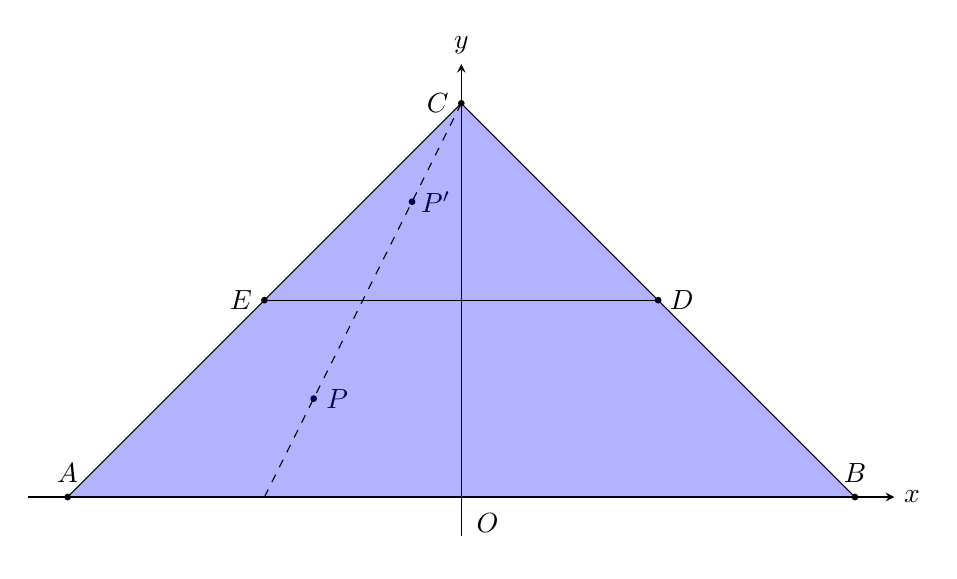
\begin{tikzpicture}
        \tzaxes(-5.5,-0.5)(5.5,5.5){$x$}{$y$}
        
        \node[circle] (o) at (1/3,-1/3){$O$};
        
        \node[circle] (o) at (-5,0.3){$A$};
        \fill[draw] (-5,0) circle (1pt) coordinate (mark-1);

        \node[circle] (o) at (5,0.3){$B$};
        \fill[draw] (5,0) circle (1pt) coordinate (mark-2);

        \node[circle] (o) at (-0.3,5){$C$};
        \fill[draw] (0,5) circle (1pt) coordinate (mark-3);

        \node[circle] (o) at (2.8,2.5){$D$};
        \fill[draw] (2.5,2.5) circle (1pt) coordinate (mark-4);

        \node[circle] (o) at (-2.8,2.5){$E$};
        \fill[draw] (-2.5,2.5) circle (1pt) coordinate (mark-5);

        \node[circle] (o) at (-0.325,3.75){$P'$};
        \fill[draw] (-0.625,3.75) circle (1pt) coordinate (mark-6);

        \node[circle] (o) at (-1.575,1.25){$P$};
        \fill[draw] (-1.875,1.25) circle (1pt) coordinate (mark-7);

        \fill[opacity=0.3,blue] (mark-1) --  (mark-2) -- (mark-3) -- cycle;

        \draw (mark-1) -- (mark-2) -- (mark-3) -- cycle;

        \draw (mark-4) -- (mark-5);

        \draw[dashed] (mark-3) -- (-2.5,0);

    \end{tikzpicture}
\end{document}